\documentclass[times, utf8, diplomski]{fer}
\usepackage{booktabs}
\usepackage[section]{placeins}

\usepackage{listings}
\lstset{
  basicstyle=\ttfamily,
  mathescape,
  extendedchars=true,
  literate={ć}{{\'c}}1 {č}{{\v{c}}}1 {đ}{{\-d}}1 {š}{{\v{s}}}1 {ž}{{\v{z}}}1
}

\graphicspath{ {./img} }

\begin{document}

\thesisnumber{1709}

\title{Detekcija osoba temeljena na konvolucijskim modelima}

\author{Domagoj Krivošić}

\maketitle

% Ispis stranice s napomenom o umetanju izvornika rada. Uklonite naredbu \izvornik ako želite izbaciti tu stranicu.
\izvornik

% TODO: Dodavanje zahvale ili prazne stranice. Ako ne želite dodati zahvalu, naredbu ostavite radi prazne stranice.
\zahvala{}

\tableofcontents

\chapter{Uvod}
Problem detekcije objekata odnosi se na pronalaženje objekta na slici, tj. određivanje lokacije objekta, te svrstavanje objekta u jedan od predefiniranih razreda. Lokacija objekta se najčešće prikazuje najmanjim pravokutnikom unutar kojeg se nalazi cijeli objekt.
U ovom radu su algoritmi za detekciju objekata podijeljeni u dvije skupine: algoritmi za detekciju koji nisu temeljeni na konvolucijskim mrežama i algoritmi za detekciju temeljeni na konvolucijskim mrežama.
Na početku su opisani algoritmi za detekciju objekata koji nisu temeljeni na konvolucijskim mrežama te je detaljnije opisan jedan algoritam kao predstavnik skupine.
Budući da je većina danas popularnih algoritama za detekciju objekata temeljena na konvolucijskim mrežama, u radu se opisuju konvolucijske mreže te operacije konvolucije i sažimanja koje su sastavni dijelovi konvolucijskih mreža. Zatim je detaljnije opisano nekoliko danas popularnih algoritama za detekciju objekata. 
U poglavlju "Opis alata", opisani su programski alati korišteni za provođenje eksperimenata i računalni resursi na kojima su se algoritmi izvodili.
Nakon teorijskog uvoda, algoritmi temeljeni na konvolucijskim mrežama su primijenjeni na zadatak detekcije osoba na označenim skupovima podataka i dan je pregled i usporedba rezultata i performansi algoritama.
Na kraju razmatramo detekciju igrača na snimkama nogometnih utakmica i komentiramo dobivene rezultate.

\chapter{Detekcija objekata prije konvolucijskih modela}
% TODO: Detekcija objekata prije konvolucijskih modela
Uvod o metodama detekcije objekata prije popularizacije konvolucijskih modela.

\section{Viola-Jones}
\cite{Viola01rapidobject} osmislili su prvi algoritam za detekciju objekata koji je radio u stvarnom vremenu. Originalno je razvijen za detekciju lica, ali moguće ga je trenirati za detekciju bilo koje vrste objekata. Tri novosti koje je algoritam donio u odnosu na prijašnje algoritme su novi način prikaza slike, algoritam za učenje temeljen na AdaBoostu i kombiniranje više klasifikatora u kaskadu počevši od jednostavnijih prema složenijima.

Algoritam radi tako da klizeći prozor prolazi po slici i za svaki prozor određuje nalazi li se objekt u njemu. Nakon svakog prolaza cijele slike prozor se povećava za određeni faktor i postupak se ponavlja. Faktor povećanja prozora direktno utječe na performanse algoritma tako da se povećanjem faktora smanjuje vrijeme potrebno za obradu jedne slike, ali se time može pogoršati preciznost i, suprotno, smanjenjem faktora se povećava vrijeme potrebno za obradu slike, ali se preciznost detekcije može povećati.
Klasifikatori ne rade s pikselima, nego sa značajkama jer se značajkama lakše može opisati domensko znanje koje bi bilo teško naučiti iz piksela. Algoritam koristi tri vrste značajki: značajke s dva, tri i četiri pravokutnika. Značajke s dva pravokutnika se računaju tako da se unutar slike izaberu dva susjedna pravokutnika jednakih veličina, a vrijednost značajke je razlika sume piksela dvaju pravokutnika. Analogno tome se računaju i značajke s tri i četiri pravokutnika. Primjeri značajki su prikazani na slici \ref{viola-jones-znacajke}.
Navedene značajke se mogu izračunati u konstantnom vremenu ako se slika prikazuje kao integralna slika. Integralna slika na lokaciji $x, y$ sadrži sumu piksela iznad i lijevo od te točke, uključujući i tu točku. Vrijednost integralne slike na lokaciji $x, y$ je opisana formulom:
\[
	ii(x, y) = \sum\limits_{x' \leq x, y' \leq y} i(x', y')
\]
, gdje je $ii(x, y)$ integralna slika, a $i(x, y)$ originalna slika. Integralna slika se iz originalne slike može izračunati u linearnoj vremenskoj složenosti. Koristeći navedeni prikaz slike, suma piksela bilo kojeg pravokutnika unutar slike se može odrediti dohvaćanjem najviše četiri vrijednosti. Primjer izračuna sume piksela unutar pravokutnika prikazan je na slici \ref{viola-jones-pravokutnici}. Ukupan broj značajki koji se može dobiti opisanim postupkom za svaki prozor veličine $24 \times 24$ je veći od $160.000$ što je puno veće od broja piksela u prozoru. Iako je izračunavanje jedne značajke jeftina operacije, izračunavanje svih značajki je skupo i nije praktično za rad u stvarnom vremenu. Pretpostavka algoritma, koja je potvrđena eksperimentima, je da se mali podskup značajki može iskoristiti za izgradnju dobrog klasifikatora. Za odabir podskupa značajki i treniranje klasifikatora koristi se varijanta algoritma AdaBoost.

\begin{lstlisting}
Pseudokod algoritma AdaBoost:
  - Skup podataka za trening s n primjera $(x_1, y_1),...,(x_n, y_n)$,
    gdje je $y_i=0$ za negativne primjere, a $y_i=1$ za pozitivne
  - Inicijaliziraj: $w_{1, i}=\frac{1}{2m}$ za $y_i = 0$ i $w_{1, i}=\frac{1}{2l}$ za $y_i = 1$,
    gdje je $m$ broj negativnih primjera, a $l$ broj pozitivnih
  - ZA $t = 1,...,T$:
      1. Normaliziraj težine tako da $w_t$ bude vjerojatnosna 
         razdioba: $w_{t, i} \gets \frac{w_{t, i}}{\sum\limits_{j=1}^{n} w_{t,j}}$
      2. Za svaku značajku j, treniraj klasifikator $h_j$ koji
         koristi samo jednu značajku. Greška se računa kao:
           $\epsilon _j = \sum\limits_i w_i|h_j(x_i) - y_i| $
      3. Izaberi klasifikator $h_t$ s najmanjom greškom $\epsilon _t$
      4. Ažuriraj težine:
           $w_{t+1, i} = w_{t, i} \beta _t^{1-e_i}$
         gdje je $e_i = 0$ ako je $x_i$ točno klasificiran,
         a $e_i = 1$ inače i $\beta _t = \frac{\epsilon _t}{1 - \epsilon _t}$
  - Konačni klasifikator je:
\end{lstlisting}
\[
	h(x) = 
	\begin{cases}
	 1, \quad za \quad  \sum\limits_{t=1}^{T} \alpha _t h_t(x) \geq \frac{1}{2} \sum\limits_{t=1}^{T} \alpha _t, \quad \alpha _t = \log{\frac{1}{\beta _t}} \\ 
	 0,	\quad inace
	\end{cases}
\]

Dobiveni klasifikatori se kombiniraju u kaskadu tako da se na početku nalaze jednostavniji klasifikatori koji koriste mali broj značajki, a na kraju složeniji koji za klasifikaciju koriste veći broj značajki. Ako jedan klasifikator prozor označi kao negativan, tj. odredi da se u njemu ne nalazi traženi objekt, prozor se odbacuje i ne prolazi kroz složenije klasifikatore. Ako, s druge strane, klasifikator označi prozor kao pozitivan, on se prosljeđuje sljedećem, složenijem klasifikatoru. Ako su svi klasifikatori označili prozor kao pozitivan, zaključujemo da se traženi objekt nalazi u tom prozoru. Opisani postupak skiciran je na slici \ref{viola-jones-kaskada}. Ideja povezivanja klasifikatora u kaskadu je da jednostavniji klasifikatori odbace veći broj prozora za koje se lako može odrediti da ne sadrže traženi objekt te se time smanji ukupni broj značajki koje je potrebno izračunati. Samo se prozori za koje nije moguće na temelju manjeg broja značajki odrediti da ne sadrže objekt prosljeđuju složenijim klasifikatorima kako bi se postigla veća točnost. Time se postiže ravnoteža između brzine izvođenja i točnosti detekcije.
Za određivanje broja značajki klasifikatora koristi se jednostavan postupak koji se temelji na činjenici da se u kaskadi svakim korakom smanjuje broj lažno pozitivnih primjera i broj detektiranih primjera. Na početku svakog koraka se postavi cilj za minimalno smanjenje lažno pozitivnih primjera i maksimalno smanjenje broja detekcija. Zatim se klasifikator trenira s određenim brojem značajki te mu se dodaju nove značajke sve dok se ne postigne postavljeni cilj. Postupak se ponavlja za svaki klasifikator.
Nakon obrade cijele slike, objekti će uglavnom biti detektirani više puta. Višestruke detekcije se rješavaju tako da se prvo sve detekcije podijele u disjunktne skupove. Dvije detekcije su u istom skupu ako se njihovi prozori preklapaju. Konačna detekcija se dobije tako da se izračuna prosjek koordinata kuteva svih prozora u skupu.

\begin{figure}
	\centering
	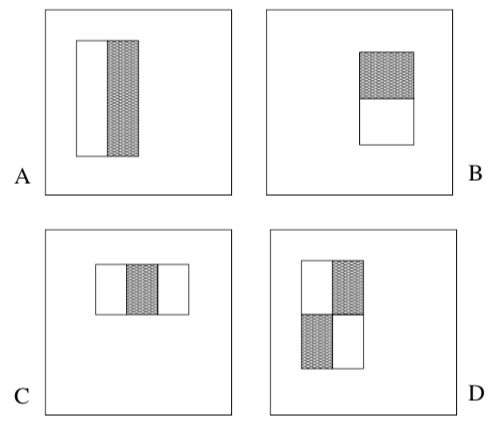
\includegraphics[scale=1]{img/viola-jones-znacajke.png}
	\caption{Primjeri značajki s dva (slike A i B), tri (slika C) i četiri (slika D) pravokutnika. Sume piksela u bijelim pravokutnicima se oduzimaju od sume piksela u sivim pravokutnicima da bi se dobila vrijednost značajke.}
	\label{viola-jones-znacajke}
\end{figure}

\begin{figure}
	\centering
	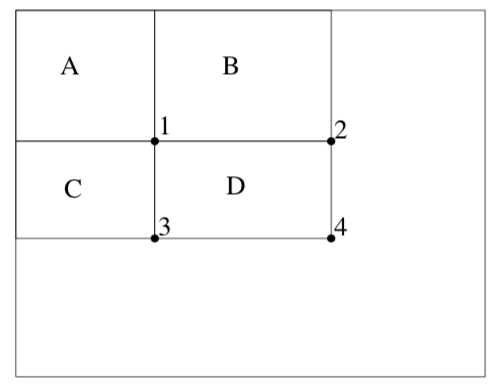
\includegraphics[scale=1]{img/viola-jones-pravokutnici.png}
	\caption{Svaka točka sadrži sumu svih piksela iznad i lijevo od sebe. Točka 1 sadrži sumu piksela unutar pravokutnika A, točka 2 sumu A + B, točka 3 sumu A + C i točka 4 sumu A + B + C + D. Za izračunavanje sume piksela unutar pravokutnika D trebaju nam vrijednosti točaka 1-4 pa sumu možemo izračunati kao $ii(4)$ - ii(3) - ii(2) + ii(1).}
	\label{viola-jones-pravokutnici}
\end{figure}

\begin{figure}
	\centering
	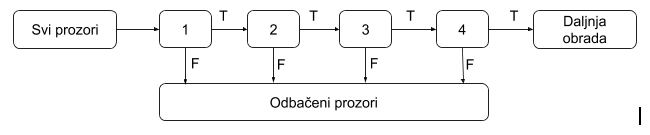
\includegraphics[scale=0.6]{img/viola-jones-kaskada.png}
	\caption{Shematski prikaz kaskade klasifikatora. Klasifikatori su označeni brojevima 1-4 i poredani po složenosti gdje je klasifikator 1 najjednostavniji, a klasifikator 4 najsloženiji. Prozor se odbacuje ako ga bilo koji klasifikator označi kao negativnog.}
	\label{viola-jones-kaskada}
\end{figure}

\chapter{Detekcija objekata konvolucijskim modelima}
Konvolucijske neuronske mreže imaju važnu ulogu u povijesti dubokog učenja jer su prvi duboki modeli koji su postigli dobre rezultate bili upravo konvolucijski modeli. Razvojem računala, osobito grafičkih procesora, konvolucijski modeli postaju sve popularniji i postižu sve bolje rezultate. Danas se većina popularnih modela za detekciju objekata temelji na konvolucijskim mrežama. U nastavku poglavlja dan je teorijski pregled konvolucijskih mreža i nakon toga je opisano nekoliko modela za detekciju objekata temeljenih na konvolucijskim mrežama.

\section{Konvolucijske mreže}
\nocite{Goodfellow-et-al-2016}

Konvolucijske neuronske mreže su posebna vrsta neuronskih mreža za obradu podataka koji imaju strukturu rešetke. Podaci koji su primjereni za obradu konvolucijskim mrežama mogu biti jednodimenzionalne rešetke, kao na primjer zvuk ili očitanja senzora u određenim vremenskim intervalima, dvodimenzionalne rešetke, kao što su slike, ili trodimenzionalne rešetke, kao što su video zapisi. Međutim, najbolji rezultati s konvolucijskim mrežama postignuti su u primjenama na slikama.
Ime konvolucijskih neuronskih mreža dolazi od matematičke operacije konvolucije koja se u njima koristi pa se i konvolucijske mreže mogu definirati kao neuronske mreže koje u barem jednom sloju umjesto množenja matrica koriste konvoluciju. U nastavku su opisane operacija konvolucije i operacija sažimanja, koja se u praksi često koristi zajedno s konvolucijom.

\subsection{Konvolucija}
Konvolucija je operacija nad dvije funkcije realne varijable. Kao primjer korištenja konvolucije možemo promatrati svemirski brod čiju lokaciju pratimo laserskim senzorom. Izlaz senzora je pozicija svemirskog broda u trenutku $t$ te ju označavamo s $x(t)$. Očitanje senzora možemo dobiti u bilo kojem trenutku t.
Pretpostavimo da su mjerenja senzora pokvarena šumom. Kako bi smanjili utjecaj šuma na očitanje, usrednjit ćemo nekoliko mjerenja s time da ćemo veću težinu dati mjerenju u trenutku $t$. To možemo postići funkcijom težine $w(a)$, gdje je $a$ starost mjerenja. Ako cjelobrojne takav težinski prosjek na mjerenje u svakom trenutku, dobijemo novu funkciju $s$ koja nam daje zaglađenu procjenu pozicije broda u trenutku $t$:
\[
s(t) = \int x(a)w(t-a)da
\]
Time smo definirali konvoluciju. Konvolucija se označava zvjezdicom:
\[
s(t) = (x \ast w)(t)
\]
U primjeru sa svemirskim brodom, $w$ mora biti funkcija gustoće vjerojatnosti da bi izlaz bio težinski prosjek. Također, $w$ mora biti jednak nuli za sve negativne argumente jer bismo u protivnom funkciji omogućili gledanje u budućnost za što je nemoguće dobiti podatke u promatranom trenutku. Općenito, konvolucija se može koristiti za razne primjene osim računanja težinskog prosjeka i definirana je za sve funkcije za koje je integral konvolucije definiran.
Kod konvolucijskih neuronskih mreža, funkciju $x$ zovemo ulaz, funkciju $w$ jezgra, a izlaz se naziva mapa značajki.
U primjeru svemirskog broda smo pretpostavili da je u svakom realnom trenutku $t$ moguće dobiti mjerenje senzora, međutim kod stvarnih mjerenja, podaci će biti dostupni u određenim vremenskim intervalima. Varijabla $t$ tada može poprimiti samo cjelobrojne vrijednosti pa možemo definirati diskretnu konvoluciju:
\[
s(t) = (x \ast w)(t) = \sum\limits_{a = - \infty}^{\infty} x(a)w(t-a) 
\] 
U velikom broju primjena neuronskih mreža, ulazi su višedimenzionalni nizovi (tenzori) podataka, a jezgre su u tom slučaju tenzori parametara. Budući da nemamo informacija o podacima koji nisu zapisani u ulaznim tenzorima, u većini slučajeva pretpostavljamo da su oni jednaki nuli, što nam olakšava implementaciju jer tada umjesto beskonačne sume trebamo izračunati sumu konačnog broja elemenata tenzora. U primjenama gdje su ulazni podaci višedimenzionalni, konvoluciju računamo istovremeno preko više osi, višedimenzionalnom jezgrom. Na primjer, kod slika imamo dvodimenzionalni ulaz pa koristimo i dvodimenzionalnu jezgru $K$. Konvoluciju tada računamo kao:
\[
S(i, j) = (I \ast K)(i, j) = \sum\limits_{m} \sum\limits_{n} I(m, n)K(i - m, j - n)
\]
Konvolucija je komutativna operacija pa se može zapisati i kao:
\[
S(i, j) = (I \ast K)(i, j) = \sum\limits_{m} \sum\limits_{n} I(i - m, j - n)K(m, n)
\]
čime smo jezgru okrenuli s obzirom na ulaz. 
Budući da u praksi komutativnost nije važno svojstvo, često se umjesto konvolucije koristi unakrsna korelacija ili neobrnuta konvolucija:
\[
S(i, j) = (I \ast K)(i, j) = \sum\limits_{m} \sum\limits_{n} I(i + m, j + n)K(m, n)
\]
U kontekstu strojnog učenja, optimizacijski algoritam će naučiti iste parametre jezgre ako koristi konvoluciju ili unakrsnu korelaciju samo na različitim mjestima. Za konvoluciju i unakrsnu korelaciju se često koristi zajednički naziv konvolucija. Slika \ref{konvolucija} prikazuje primjer izračuna unakrsne korelacije za dvodimenzionalni ulaz veličine $3 \times 3$ i dvodimenzionalnu jezgru veličine $2 \times 2$.

 \begin{figure}
	\centering
	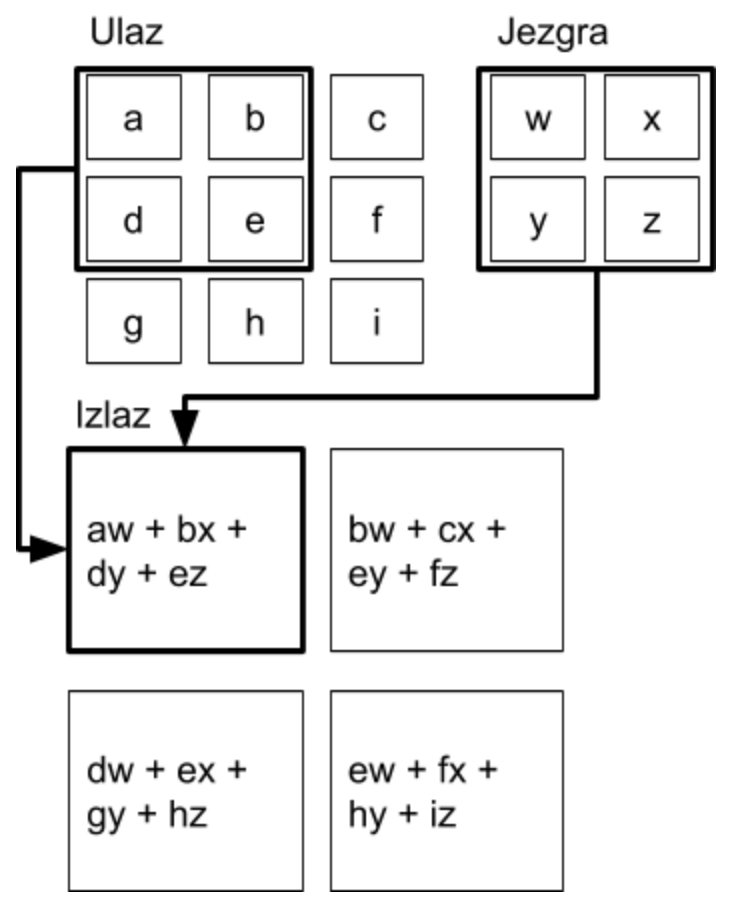
\includegraphics[scale=0.6]{img/konvolucija.png}
	\caption{Primjer konvolucije. Prozor veličine jezgre se pomiče po ulaznom tenzoru te se svaki element unutar prozora u ulaznom tenzoru množi s odgovarajućim elementom jezgre, a dobivene vrijednosti se zbrajaju. Za svaki pomak prozora se na izlazu dobije jedan broj.}
	\label{konvolucija}
\end{figure}

\subsection{Prednosti konvolucije}
Konvolucija koristi tri važne ideje koje poboljšavaju performanse neuronske mreže: rijetku povezanost, dijeljenje parametara i reprezentaciju ekvivarijantnu s obzirom na pomak. 
Slojevi potpuno povezanih neuronskih mreža množe matricu izlaza prethodnog sloja s matricom parametara gdje svaki element matrice parametara modelira vezu jednog ulaznog neurona s jednim izlaznim neuronom. To znači da ako prethodni sloj ima $m$ neurona, a trenutni $n$ parametara, matrica parametara trenutnog sloja mora biti dimenzija $m \times n$ i vremenska složenost izračuna izlaza sloja je $O(m \times n)$.
Za razliku od potpuno povezanih slojeva, konvolucijski slojevi su rijetko povezani, a to se postiže odabirom jezgre koja je manjih dimenzija od ulaza. Na primjer, slike mogu imati milijune piksela, a jezgra od nekoliko desetaka ili stotina piksela može biti dovoljna za naučiti korisne značajke. Ako broj veza izlaznog sloja ograničimo na $k$, gdje je $k \ll m$, prostorna i vremenska složenost će biti $O(k \times n)$. U praksi je moguće postići dobre rezultate koristeći $k$ koji je nekoliko redova veličine manji od $m$.
Dijeljenje parametara se odnosi na korištenje istih parametara za modeliranje više veza između ulaznih i izlaznih neurona. U potpuno povezanim slojevima, svaki težina se koristi samo jednom dok se kod konvolucijskih mreža svaki element jezgre koristi na svakoj poziciji ulaza. Dijeljenjem parametara postižemo da umjesto učenja novih parametara za svaku lokaciju ulaza, učimo samo jedan skup parametara što ne utječe na brzinu izvođenja, ali smanjuje broj parametara na $k$.
Rijetka povezanost i dijeljenje parametara omogućuju konvolucijskim mrežama rad s ulazima različitih veličina.
Razlike između potpuno povezanog sloja, rijetko povezanog sloja i rijetko povezanog sloja s dijeljenjem parametara ilustrirane su slikom \ref{povezanost}.
Posljedica dva opisana principa je svojstvo koje se zove ekvivarijantnost na pomak. Funkcija je ekvivarijantna ako se promjenom ulaza, izlaz mijenja na isti način, tj. ako vrijedi $f(g(x)) = g(f(x))$. Na primjer, neka je $I$ funkcija koja za zadane koordinate vraća svjetlinu slike i neka je $g$ funkcija koja pomiče svaki piksel slike za jedan u desno i vraća novu, translatiranu sliku $I' = g(I)$, gdje je $I'(x, y) = I(x-1, y)$. Napravimo li transformaciju $g$ na slici I i zatim nad dobivenom slikom primprimijenimojenimo konvoluciju, dobit ćemo isti rezultat kao da smo prvo primijenili konvoluciju nad slikom $I$, a zatim napravili transformaciju dobivenog izlaza. Svojstvo ekvivarijantnosti na pomak je korisno kada znamo da se slični ili isti uzorci mogu pojaviti na više mjesta u slici pa dijeljenje parametara omogućava da se jednom naučeni uzorci mogu prepoznati na bilo kojem mjestu u slici, bez obzira je li uzorak na tom mjestu viđen prilikom treninga ili nije. Primjer u kojem je ovo svojstvo važno je detekcija objekata. 
Konvolucija međutim nije ekvivarijantna s obzirom na skaliranje i rotaciju.

 \begin{figure}
	\centering
	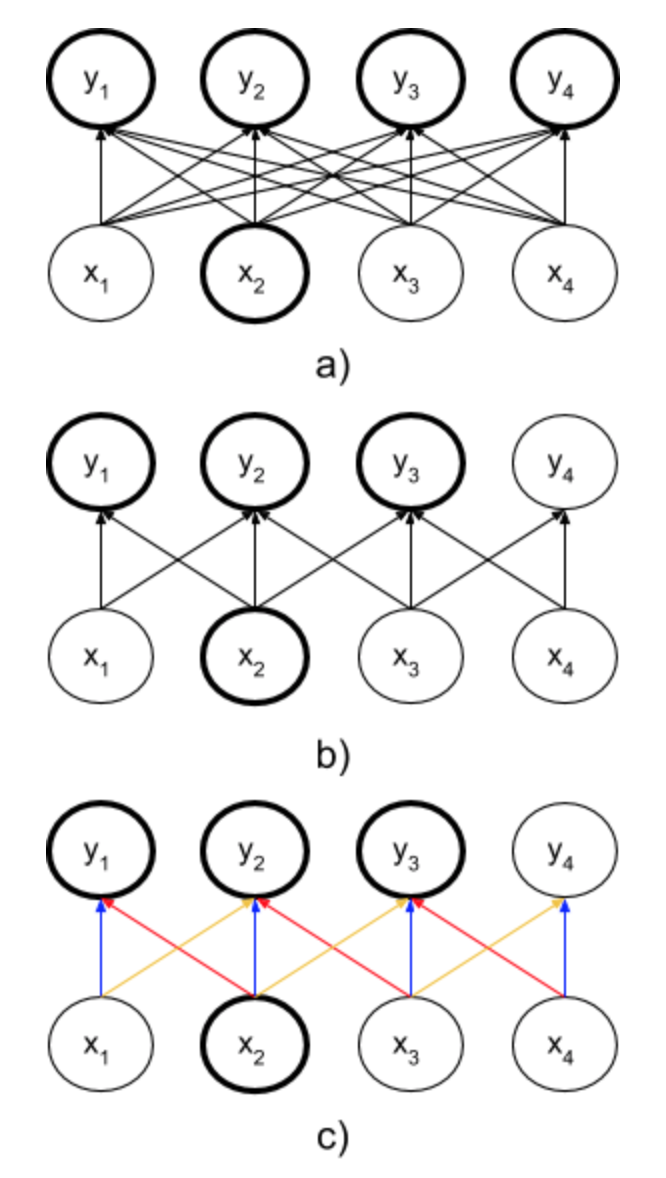
\includegraphics[scale=0.8]{img/povezanost.png}
	\caption{Slika a) prikazuje dva potpuno povezana sloja neuronske mreže. Svaki neuron u jednom sloju, povezan je sa svim neuronima drugog sloja. Težina veze između svaka dva neurona je poseban parametar pa zadani primjer ima 16 parametara. Slika b) prikazuje dva rijetko povezana sloja. Svaki neuron u jednom sloju je povezan samo s određenim brojem neurona u drugom sloju. Svaka veza dva neurona je poseban parametar pa je ukupan broj parametara 10. Slika c) prikazuje dva rijetko povezana sloja s dijeljenim parametrima. Veze između neurona označene istom bojom su isti parametri pa je ukupan broj parametara 3.}
	\label{povezanost}
\end{figure}

\subsection{Sažimanje}
Tipični konvolucijski sloj se sastoji od konvolucije, nelinearne aktivacijske funkcije i sloja sažimanja. Sloj sažimanja preslikava skup prostorno bliskih značajki na ulazu u jednu značajku na izlazu pri čemu je izlaz uglavnom neki statistički pokazatelj kao npr. srednja vrijednost ili maksimum. Općenito, sažimanjem se postiže invarijantnost na pomak što znači da ako se ulaz translatira za mali iznos, većina vrijednosti na izlazu sloja sažimanja će ostati nepromijenjena. Invarijantnost na male translacije je posebno korisna ako nas ne zanima točan položaj neke značajke, nego samo pojavljuje li se ta značajka ili ne. Budući da se sažimanjem dobije statistička mjera cijelog susjedstva, na izlazu možemo koristiti i manji broj značajki od samog broja ulaza. Kako bi se izbjeglo računanje izlaza koji se ne koriste, izlaze možemo računati tako da se pri računanju izlaza sloja sažimanja pomičemo za $k$ piksela umjesto za jedan. Time se postiže i veća brzina izvođenja jer se broj izračuna smanji za otprilike $k$ puta. Sažimanje je u mnogim primjenama važno za obradu ulaza različitih veličina. Na primjer, kod klasifikacije slika, potpuno povezani slojevi moraju imati fiksan ulaz pa se reguliranjem pomaka i veličine sloja sažimanja može osigurati da je izlaz iz sloja uvijek fiksne veličine. 

 \begin{figure}
	\centering
	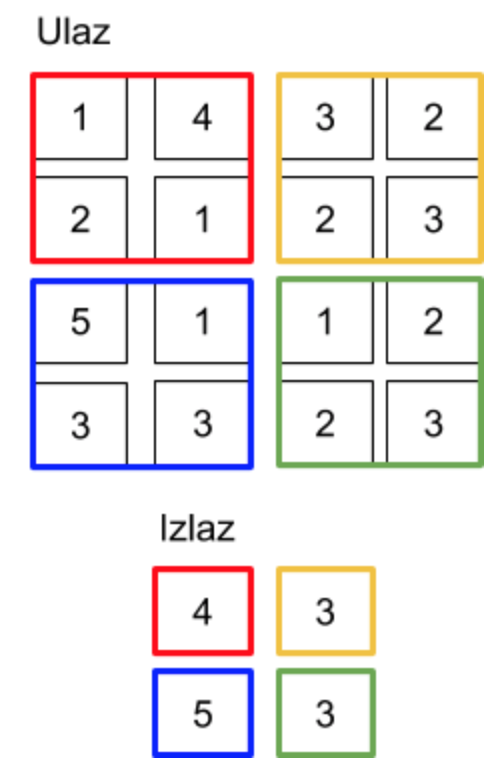
\includegraphics[scale=1]{img/sazimanje.png}
	\caption{Sažimanje maksimalnom vrijednosti s pomakom od 2 piksela.}
	\label{sazimanje}
\end{figure}


\section{R-CNN}
Prvi model za detekciju objekata zasnovan na konvolucijskim mrežama koji ćemo opisati je Regions with CNN features ili R-CNN (\cite{DBLP:journals/corr/GirshickDDM13}). Na skupu podataka VOC2012 je postigao 30\% veću prosječnu preciznost od prethodno najboljih modela. 
R-CNN sustav za detekciju objekata se sastoji od tri dijela. Detekcija R-CNN modelom ilustrirana je na slici \ref{rcnn}. Prvi dio generira prijedloge regija u kojima bi se mogao nalaziti objekt. Za predlaganje regija se može koristiti bilo koja metoda, ali autori koriste selektivnu pretragu kojom generiraju oko 2000 regija za svaku sliku.
Nakon toga se svaka regija šalje u drugi dio modela, duboku konvolucijsku mrežu, koja na izlazu daje 4096-dimenzionalni vektor dubokih značajki. Arhitektura mreže nije strogo definirana pa se može izabrati proizvoljno, ali izbor arhitekture u velikoj mjeri utječe na performanse modela. Konvolucijska mreža na ulazu očekuje RGB sliku dimenzija $227 \times 227$ u kojoj je vrijednostima piksela oduzeta srednja vrijednost piksela. Budući da su regije proizvoljnih veličina, prije prosljeđivanja regije konvolucijskoj mreži, mijenjaju joj se dimenzije na $227 \times 227$ bez obzira na omjer visine i širine. Prije mijenjanja dimenzija regije, prozor koji određuje regiju se proširuje za 16 piksela sa svake strane.
Treći dio modela čine binarni klasifikatori koji klasificiraju vektor dubokih značajki u neki od razreda. Za svaki razred se trenira jedan SVM koji označava regiju kao pozitivnu ili negativnu. Ako svi klasifikatori označe regiju kao negativnu, regija se smatra pozadinom.
Na kraju se svaka detekcija dovodi na ulaz jednostavnom modelu koji za predloženu regiju predviđa konačni prozor u kojem se nalazi objekt kako bi se poboljšala točnost detekcije.
Svaka komponenta modela se trenira posebno. Skup podataka za trening sastoji se od slika, regija predloženih selektivnom pretragom i konačnih detekcija s klasama objekata.
Konvolucijska mreža se predtrenira na skupu podataka za klasifikaciju slika, a zatim se trening nastavlja za klasifikaciju predloženih regija. Ako je omjer presjeka i unije predložene regije i stvarnog prozora u kojem se nalazi objekt veći od određenog praga (npr. 0.3), regija se klasificira kao da sadrži objekt, inače se klasificira kao pozadina.
Nakon treninga konvolucijske mreže, treniraju se klasifikatori (SVM), po jedan za svaki razred. Za trening klasifikatora se koriste duboke značajke dobivene iz regije konvolucijskom mrežom. Razredi regija se određuju na isti način kao i kod treninga konvolucijske mreže.
Modeli koji predviđaju konačne koordinate prozora se treniraju posebno za svaki razred. Za njihov trening se koriste predviđene regije kao ulazni podaci i stvarne lokacije objekata kao očekivani izlazi.

 \begin{figure}
	\centering
	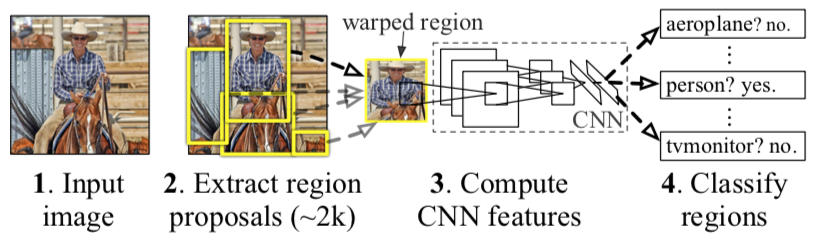
\includegraphics[scale=1]{img/rcnn.png}
	\caption{Vizualizacija detekcije R-CNN modelom.}
	\label{rcnn}
\end{figure}



\section{Fast R-CNN}
R-CNN postiže dobre rezultate na problemu detekcije objekata, ali ima nekoliko velikih nedostataka. Treniranje modela je komplicirano jer se svaka komponenta trenira zasebno. Također, treniranje je vremenski i memorijski vrlo zahtjevno jer je za trening klasifikatora potrebno dobiti duboke značajke za sve slike i spremiti ih na disk što je posebno izraženo pri korištenju većih konvolucijskih mreža. Treći veliki nedostatak je sporost detekcije objekata jer je i kod predikcije potrebno za svaku predloženu regiju izlučiti duboke značajke da bi se regija mogla klasificirati.
Fast R-CNN (\cite{DBLP:journals/corr/Girshick15}) donosi nekoliko poboljšanja u odnosu na R-CNN. Cijeli model se trenira odjednom, nema potrebe za privremenim pohranjivanjem dubokih značajki i postiže veću preciznost detekcije.
Arhitektura modela prikazana je na slici \ref{fast_rcnn}. Na ulazu Fast-RCNN mreža prima sliku i skup predloženih regija u kojima se potencijalno nalazi objekt. Mreža prvo računa mapu dubokih značajki za cijelu sliku koristeći duboku konvolucijsku mrežu koja se sastoji od nekoliko konvolucijskih slojeva i nekoliko slojeva sažimanja maksimalnom vrijednošću. Nakon toga se, za svaku predloženu regiju, iz dobivene mape značajki izlučuje vektor značajki konstantne duljine korištenjem RoI (Region of Interest) sloja sažimanja. Svaki vektor značajki se zatim prosljeđuje potpuno povezanim slojevima koji se na kraju granaju u dva izlazna sloja: jedan sa softmax aktivacijskom funkcijom koji procjenjuje vjerojatnosti pripadnosti regije svakom od $K + 1$ razreda (K razreda objekata i jedan dodatni koji predstavlja pozadinu) i drugi, koji na izlazu daje četiri broja za svaki razred koji opisuju prozor u kojem se nalazi objekt. 
RoI sloj sažimanja koristi sažimanje maksimalnom vrijednošću kako bi na izlazu vratio vektor značajki konstantne veličine $H \times W$. Izlazni vektor se računa tako da se ulazni prozor dimenzija $h \times w$ podijeli u mrežu dimenzija $H \times W$, gdje je veličina svake ćelije mreže $\frac{h}{H} \times \frac{w}{W}$ te se u svakoj ćeliji odredi maksimalna vrijednost.
Važno svojstvo Fast R-CNN modela je da se sve težine mogu trenirati backpropagation algoritmom. Budući da model ima dva izlazna sloja, a ostali slojevi su dijeljeni, funkcija pogreške uključuje pogrešku oba izlazna sloja:
\[
L(p, u, t^u , v) = L_{cls}(p, u) + \lambda [u \geq 1]L_{loc}(t^u, v)
\]
, gdje je $p$ vjerojatnosna razdioba na izlazu sloja sa softmax aktivacijskom funkcijom $p = (p_0, ..., p_K)$, $u$ je stvarni razred regije na ulazu, $t^k$ je predviđeni prozor, a $v$ je stvarni prozor u kojem se nalazi objekt. Izraz $[u \geq 1]$ ima vrijednost 1 ako je stvarni razred objekta neki $1...K$, a 0 ako je stvarni razred objekta 0. Razred 0 označava pozadinu pa u tom slučaju nema smisla određivati lokaciju objekta. Za pogrešku klasifikacije se koristi negativna log-izglednost stvarnog razreda $u$ $L_{cls}(p, u) = - \log p_u$, a za pogrešku lokalizacije objekta se koristi zaglađena $L_1$ pogreška
\[
L_{loc}(t^u, v) = \sum\limits_{i \epsilon \{ x, y, w, h \}} smooth_{L_1} (t^u_i - v_i)
\]
, gdje je
\[
smooth{L_1}(x) = 
	\begin{cases}
		0.5x^2, \quad \quad za \quad |x| < 1 \\
		|x| - 0.5, \quad inace
	\end{cases}
\]

Funkcija pogreške koja uključuje pogreške oba izlazna sloja ima i veću preciznost u odnosu na model koji je odvojeno treniran za klasifikaciju i regresiju.
Da bi se postigla invarijantnost na skalu, koristi se metoda svođenja slika na istu skalu, gdje se skala definira kao duljina kraće stranice.
U usporedbi s R-CNNom, Fast R-CNN donosi poboljšanje u preciznosti detekcije i velika ubrzanja u treningu i detekciji objekata.

 \begin{figure}
	\centering
	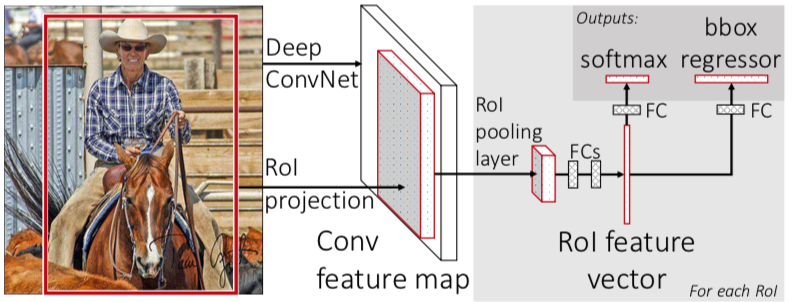
\includegraphics[scale=1]{img/fast_rcnn.png}
	\caption{Arhitektura Fast R-CNN.}
	\label{fast_rcnn}
\end{figure}

\section{Faster R-CNN}
% TODO: Faster R-CNN
Opis algoritma.

\section{R-FCN}
% TODO: R-FCN
Opis algoritma

\section{YOLO}
% TODO: YOLO
Opis algoritma.

\section{Single Shot MultiBox Detector}
% TODO: SSD
Opis algoritma.

\chapter{Opis alata}
% TODO: Opis alata
Opis tensorflow object detection API frameworka i strukture projekta.

\chapter{Rezultati}
% TODO: Rezultati
Rezultati postignuti na različitim skupovima slika i primjeri.



\chapter{Zaključak}
% TODO: Zaključak
Zaključak.


\bibliography{literatura}
\bibliographystyle{fer}

\begin{sazetak}
% TODO: Sazetak
Sažetak na hrvatskom jeziku.

\kljucnerijeci{Ključne riječi, odvojene zarezima.}
\end{sazetak}

\engtitle{Person Detection Based on Convolutional Models}
\begin{abstract}
% TODO: Abstract
Abstract.

\keywords{Keywords.}
\end{abstract}

\end{document}
